%%%%%%%%%%%%%%%%%%%%%%%%%%%%%%%%%%%%%%%%%%%%%%%%%%%%%%%%%%%%%%%%%%%%%%%%
% Copyright (c) 2022 Antonio Coín Castro
%
% This work is licensed under a
% Creative Commons Attribution-ShareAlike 4.0 International License.
%
% You should have received a copy of the license along with this
% work. If not, see <http://creativecommons.org/licenses/by-sa/4.0/>.
%%%%%%%%%%%%%%%%%%%%%%%%%%%%%%%%%%%%%%%%%%%%%%%%%%%%%%%%%%%%%%%%%%%%%%%%

\section{Bayesian methodology for RKHS-based functional regression models}\label{sec:methodology}

In this section we present the precise models and Bayesian methodologies explored in this work. The RKHS-based functional models under consideration \citep[see][]{berrendero2018functional, berrendero2019rkhs} are those obtained by taking a functional parameter \(\alpha \in \Hcal(K)\) and replacing the scalar product for \(\dotprod{X}{\alpha}_K\) in the \(L^2\)-models~\eqref{eq:l2-linear-model} and~\eqref{eq:l2-logistic-model}. However, to further simplify things we will follow a parametric approach and suppose that \(\alpha\) is in fact a member of the dense subspace \(\Hcal_0(K)\) defined in~\eqref{eq:h0}. For practical and computational reasons, the value of \(p\), the dimensionality of the model, will be fixed beforehand in a suitable way (see Section~\ref{sec:model-choice} for details), and we will regard \(\beta_j\) and \(t_j\) as free parameters. Thus, we will search for our functional parameter in the set
\begin{equation}\label{eq:h0p}
\Hcal_{0,p}(K)=\left\{ \sum_{j=1}^p \beta_j K(t_j, \cdot): \ \beta_j \in \R, \ t_j \in [0, 1]\right\}.
\end{equation}

The general idea will be to impose a prior distribution on these free parameters (and possibly others) to eventually derive a posterior model after incorporating the available sample information.  Moreover, as we said before, with a slight abuse of notation we will understand the expression \(\dotprod{x}{\alpha}_K\) as \(\Psi_x(\alpha)\), where \(x=X(\omega)\) and \(\Psi_x\) is Loève's isometry. Hence, taking into account that \(\alpha \in \Hcal_{0,p}(K)\) and that \(\Psi_X(K(t, \cdot)) = X(t)\) by definition (see~\eqref{eq:loeves-isometry}), we can write \(\dotprod{x}{\alpha}_K \equiv \sum_j \beta_j x(t_j)\) when \(\alpha(\cdot)=\sum_j\beta_j K(t_j, \cdot)\).

In view of~\eqref{eq:h0p}, to set a prior distribution on the unknown function \(\alpha\) (that is, a prior distribution on the functional space \(\Hcal_{0,p}(K)\)) it suffices to consider \(p\)-dimensional continuous prior distributions for the coefficients \(\beta_j\) and the times \(t_j\) separately. Thanks to this parametric approach, the challenging task of setting a prior distribution on a space of functions is considerably simplified, while simultaneously not constraining the model to any specific distribution (in contrast to, for instance, Gaussian process regression methods). Moreover, note that starting from a probability distribution \(\mathbb{P}_0\) on \(\Hcal_0(K)\) we can obtain a probability distribution \(\mathbb{P}\) on \(\Hcal(K)\) merely by defining \(\mathbb{P}(B) = \mathbb{P}_0(B\cap \Hcal_0(K))\) for all Borel sets \(B\). Consequently, our simplifying assumption on \(\alpha\) is not very restrictive, since any prior distribution on \(\Hcal_0(K)\) can be directly extended to a prior distribution on \(\Hcal(K)\). Even though we actually work on \(\Hcal_{0,p}(K)\), the discrete parameter \(p\) can still be selected in several meaningful ways that make use of the available data, and the set of feasible values is not very large in practice.

In any case, after selecting a suitable prior distribution \(\pi(\theta)\) for the finite-dimensional parameter vector \(\theta\), we can resort to Bayes' theorem to perform the inference step, which in the case of i.i.d. samples amounts to
\begin{equation}\label{eq:bayes-theorem}
  \pi(\theta \mid \mathcal D_n) \propto \left( \prod_{i=1}^n \pi(Y_i\mid X_i, \theta) \right)\pi(\theta).
\end{equation}
In Sections~\ref{sec:rkhs-linear-model} and~\ref{sec:rkhs-logistic-model} we proceed to specify the parameter spaces, prior distributions and concrete models for \(\pi(Y | X,\theta)\) considered in the case of functional linear regression and functional logistic regression, respectively. Even though in~\eqref{eq:bayes-theorem} we have omitted the possibly intractable integral related to the normalizing constant, sampling from the (approximate) posterior distribution can be accomplished via Markov Chain Monte Carlo (MCMC) methods \citep[e.g.][]{brooks2011handbook}. Note that the use of MCMC algorithms introduces a source of stochasticity in the prediction procedure.

\subsection{Functional linear regression}\label{sec:rkhs-linear-model}

In the case of functional linear regression, the simplified RKHS model considered in this work is given by
\begin{equation}\label{eq:rkhs-model-linear}
  Y = \alpha_0 + \Psi_X(\alpha) + \epsilon = \alpha_0 + \sum_{j=1}^p \beta_j X(t_j) + \epsilon,
\end{equation}
where \(\alpha(\cdot)=\sum_{j=1}^p\beta_jK(t_j, \cdot) \in \Hcal_{0,p}(K), \beta_j \in \R\), \(t_j \in [0, 1]\), \(\alpha_0\in\R\), and \(\epsilon\) is a normally-distributed error term independent from \(X\), with \(\E[\epsilon]=0\) and \(\Var(\epsilon)=\sigma^2\in \R^+\). This model is essentially a finite-dimensional approximation from a functional perspective to the more general RKHS model that assumes \(\alpha \in \Hcal(K)\), proposed in~\citet{berrendero2019rkhs}.

When \(p\) is fixed, the parameter space of dimension \(2p + 2\) becomes \(\Theta_p = \R^p \times [0, 1]^p \times \R \times \R^+\), and in the sequel a generic element of this space will be denoted by \(\theta = (\beta_1,\dots, \beta_p, t_1,\dots, t_p, \alpha_0, \sigma^2) \equiv (b, \tau, \alpha_0, \sigma^2)\). Before proceeding any further, observe that we can rewrite model~\eqref{eq:rkhs-model-linear} in a more explicit and practical fashion in terms of the available sample information in \(\mathcal D_n\). For \(\theta \in \Theta_p\), the reinterpreted model assumes the form
\begin{equation}\label{eq:rkhs-model-linear-2}
  Y_i \mid X_i, \theta \ \stackrel{\text{i.i.d.}}{\sim} \mathcal N\left(\alpha_0 + \sum_{j=1}^p \beta_j X_i(t_j), \ \sigma^2\right), \quad i =1,\dots, n.
\end{equation}

It is worth mentioning that the model remains linear in the sense that it fundamentally involves a random variable belonging to the linear span of the process \(X\) in \(L^2(\Omega)\). Also, note that given the time instants \(t_j\), the model becomes a multiple linear model with the \(X(t_j)\) as scalar covariates. As a matter of fact, this RKHS model is particularly suited as a basis for variable selection methods, and also entails the classical \(L^2\)-model~\eqref{eq:l2-linear-model} under certain conditions \citep[see][Sec.~3]{berrendero2020general}. In addition, this model could be easily extended to the case of several covariates via an expression of type \(Y=\alpha_0 + \Psi_{X^{1}}(\alpha_1) + \cdots + \Psi_{X^{q}}(\alpha_q) + \epsilon\). In that case, as argued in \citet{grollemund2019bayesian} for a similar situation, if we were to set a prior distribution on all the parameters involved, we could recover the full posterior by looking alternately at the posterior distribution of each covariate conditional on the rest of them.

\subsubsection{The bayesian approach: prior selection and posterior derivation}

The prior distribution suggested for the parameter vector \(\theta \in \Theta_p\) is given by
\begin{align}\label{eq:prior-linear}
  \begin{split}
  \pi(\alpha_0, \sigma^2)              & \propto 1/\sigma^2,                                                     \\
  \tau                     & \sim \mathcal U([0, 1]^p),                                              \\
  b\mid \tau, \sigma^2 & \sim \mathcal N_p(b_0, g\sigma^2{\underbrace{\left(\mathcal X_\tau' \mathcal X_\tau + \eta I\right)}_{G_\tau}}^{-1}),
\end{split}
\end{align}
where \(I\) is the identity matrix, \(\mathcal X_\tau\) is the data matrix \((X_i(t_j))_{i,j}\), and \(b_0\in \R^p, \ g \in \R\) and \(\eta \in \R^+\) are hyperparameters of the model. On the one hand, note the use of a joint prior distribution on \(\alpha_0\) and \(\sigma^2\), which is a widely used non-informative prior known as Jeffrey's prior \citep{jeffreys1946invariant}. In any event, the estimation of \(\alpha_0=\E[Y]\) is straightforward, so it could have been left out of the model altogether. On the other hand, the prior on \(b\) is a slight modification of the well-known Zellner's g-prior \citep{zellner1986assessing}, in which a regularizing term is added to avoid ill-conditioning problems in the Gram matrix, obtaining a ridge-like Zellner prior controlled by the tuning parameter \(\eta\) \citep{baragatti2012study}. All in all, with a slight abuse of notation the proposed prior distribution becomes \(\pi(\theta) = \pi(b| \tau, \sigma^2)\pi(\tau)\pi(\alpha_0, \sigma^2)\).

As for the posterior distribution, we only compute a function proportional to its log-density, since that is all that is needed for the MCMC algorithm to work. A standard algebraic manipulation in~\eqref{eq:bayes-theorem} yields the following result.

\begin{proposition}
Under the linear model~\eqref{eq:rkhs-model-linear-2}, the prior distribution implied in~\eqref{eq:prior-linear} produces the log-posterior distribution
\begin{align*}
\log \pi(\theta \mid \mathcal D_n) \propto {} & \frac{1}{2\sigma^2}\left(\|\symbf Y- \alpha_0\symbf{1} - \mathcal X_\tau b\|^2 + \frac{1}{g}(b - b_0)'G_\tau(b - b_0) \right)\\
& + (p+n+2)\log\sigma - \frac{1}{2}\log |G_\tau|,
\end{align*}
where \(\symbf Y=(Y_1,\dots,Y_n)'\) and \(\symbf{1}\) is an \(n\)-dimensional vector of ones.
\end{proposition}

\subsubsection{Making predictions}

In order to generate predictions, let us recall that when performing the empirical posterior approximation, on each of the \(M\) steps of the iterative MCMC algorithm we get an approximate sample \(\theta^{(m)*}=(b^{(m)*}, \tau^{(m)*}, \alpha_0^{(m)*}, (\sigma^2)^{(m)*})\) of the posterior distribution \(\pi(\theta| \mathcal D_n)\). Assuming now a previously unseen test set \(\mathcal D'_{n'}\) in the same conditions as \(\mathcal D_n\), we propose to construct three different kinds of predictors based on the MCMC samples, each of them following a different strategy.

\begin{description}
  \item[Summarize-then-predict.] If we consider a point-estimate statistic \(T\) to act as a summary of the posterior distribution, we can get the corresponding estimates \(\hat{\theta}=(\hat b, \hat \tau, \hat{\alpha}_0, \hat{\sigma}^2) = T\{\theta^{(m)*}\} \equiv (T\{b^{(m)*}\}, T\{\tau^{(m)*}\}, T\{\alpha_0^{(m)*}\}, T\{(\sigma^2)^{(m)*}\})\) and predict the responses in the usual way following model \eqref{eq:rkhs-model-linear}, i.e.:
  \[
    \hat Y_i = \hat{\alpha}_0 + \sum_{j=1}^p \hat{\beta}_j X_i(\hat{t}_j), \quad i=1,\dots, n'.
  \]
  Note that in this case the variance \(\sigma^2\) is treated as a nuisance parameter. Although it contributes to measure the uncertainty in the approximations, its estimates are discarded in the final prediction.

  \item[Predict-then-summarize.] Alternatively, we can  look at the approximate posterior distribution as a whole and compute the predictive distribution of the simulated responses at each step of the chain following model~\eqref{eq:rkhs-model-linear-2}:
  \begin{equation}\label{eq:sampled-response-vector}
  \symbf Y^{(m)*} := \left\{Y_i^{(m)*} \equiv Y_i \mid X_i, \theta^{(m)*}:\ i=1,\dots,n'\right\}, \quad m=1,\dots,M.
  \end{equation}
  Then, we can take the mean of all such simulated responses as a proxy for each response variable, that is,
  \[
  \hat Y_i = \frac{1}{M}\sum_{m=1}^M Y_i^{(m)*}, \quad i=1,\dots,n'.
  \]
  This method differs from the previous one in that it takes into account the full approximate posterior distribution instead of summarizing it directly.

  \item[Variable selection.] Lastly, we can focus only on the marginal posterior distribution of \(\tau|\mathcal D_n\) and select \(p\) time instants using a point-estimate statistic \(T\) as in our first strategy, but discarding the rest of the parameters. Specifically, we can consider the times \(\hat t_j = T\{t_j^{(m)*}\}\) and reduce the original data set to just the \(n\times p\) real matrix \(\{X_i(\hat t_j): i=1, \dots,n, \ j=1,\dots,p\}\). After this variable selection has been carried out, we can tackle the problem using a finite-dimensional linear regression model and apply any of the well-known prediction algorithms suited for this situation.
\end{description}

Note that these predictors can be obtained all at once after only one round of training (that is, an individual MCMC run to approximate the posterior distribution). As a consequence, what we have in practice is a single algorithm that can produce multiple predictors at the same computational cost, so that any of them can be chosen (or even switched back and forth) depending on the particularities of the problem at hand. Moreover, one could even contemplate an \textit{ensemble model} in which some kind of aggregation of several of the available prediction methods is performed to produce a final result.

\subsection{Functional logistic regression}\label{sec:rkhs-logistic-model}

In the case of functional logistic regression, we regard the binary response variable \(Y\in\{0, 1\}\) as a Bernoulli random variable given the regressor \(X=x \in L^2[0, 1]\), and suppose that \(\log\left(p(x)/(1-p(x))\right)\) is linear in \(x\), where \(p(x)=\mathbb P(Y=1| X=x)\). Then, following the approach  suggested by \citet{berrendero2018functional}, an RKHS model might be given  by the  equation
\begin{equation}\label{eq:rkhs-model-logistic}
  \mathbb P(Y=1 \mid X) = \frac{1}{1 + \exp\{-\alpha_0 - \Psi_X(\alpha)\}}, \quad \alpha_0 \in \R, \ \alpha \in \Hcal_{0,p}(K).
\end{equation}

Indeed, note that this can be seen as a finite-dimensional approximation (but, still, with a functional interpretation) to the general RKHS functional logistic model proposed by these authors, which can be obtained by replacing \(\Hcal_{0,p}(K)\) with the whole RKHS space \(\Hcal(K)\). Now, if we aim at a classification problem, our strategy will be similar to that followed in the functional linear model: after incorporating the sample information, we can rewrite~\eqref{eq:rkhs-model-logistic} as
\begin{equation}\label{eq:rkhs-model-logistic-2}
Y_i \mid X_i,\theta \ \stackrel{\text{i.i.d.}}{\sim} \operatorname{Bernoulli}(p_i), \quad i=1,\dots, n,
\end{equation}
with
\begin{equation}\label{eq:rkhs-model-logistic-2-parameter}
  p_i = \mathbb P(Y_i=1 \mid X_i,\theta) = \frac{1}{\displaystyle 1 + \exp\left\{-\alpha_0 - \sum_{j=1}^p \beta_j X_i(t_j)\right\}}, \quad i=1,\dots, n,
\end{equation}
where in turn \(\beta_j\in\R\) and \(t_j\in[0, 1]\).

In much the same way as the linear regression model described above, this RKHS-based logistic regression model offers some advantages over the \(L^2\)-model. First and foremost, it has a more straightforward interpretation and allows for a workable Bayesian approach, as we will demonstrate below. Secondly, it can be shown that under mild conditions the general RKHS logistic functional model holds whenever the conditional distributions \(X | Y=i\) (\(i=0,1\)) are homoscedastic Gaussian processes~\citep[see Theorem 1 in][]{berrendero2018functional}; this provides a sound theoretical motivation for such model. Furthermore, a maximum likelihood approach for parameter estimation (although not considered here) is possible as well. Indeed, the use of a finite-dimensional approximation  mitigates the problem of non-existence of the MLE in the functional case. However, let us recall that even in finite-dimensional settings there are cases of quasi-complete separation in which the MLE does not exist \citep{albert1984existence}, though this issue can be circumvented using, for example, Firth's corrected estimator \citep{firth1993bias}.
\color{black}

\subsubsection{The Bayesian approach: prior selection and posterior derivation}

As far as prior distributions go, we propose to use the same ones as we did in~\eqref{eq:prior-linear} for the linear regression model. However, in this case the parameter \(\sigma^2\) is a nuisance parameter and can be safely ignored at the end, since it does not appear in the final model. The posterior distribution is then derived after a routine calculation.

\begin{proposition}
Under the logistic model~\eqref{eq:rkhs-model-logistic-2}, the prior distribution implied in~\eqref{eq:prior-linear} produces the log-posterior distribution
\begin{align*}
  \log \pi(\theta \mid \mathcal D_n) \propto {} & \sum_{i=1}^n \left[ \left(\alpha_0 + \Psi_{X_i}(\alpha)\right)Y_i - \log\left(1 + \exp\left\{\alpha_0 + \Psi_{X_i}(\alpha)\right\}\right)\right]\\
  \quad &+ \frac{1}{2}\log |G_\tau| - (p+2)\log \sigma -\frac{1}{2g\sigma^2} (b - b_0)'G_\tau(b - b_0).
\end{align*}
Remember that \(\Psi_{X_i}(\alpha) = \sum_{j=1}^p \beta_j X_i(t_j)\).
\end{proposition}

\subsubsection{Making predictions}

Bear in mind that in this case we are essentially approximating the probabilities \(p_i\) in~\eqref{eq:rkhs-model-logistic-2-parameter}, so before producing a response we need to transform the predicted values to a binary output in \(\{0, 1\}\). According to the usual criterion of minimizing the misclassification probability, the Bayes optimal rule is recovered by predicting \(\hat Y=1\) whenever \(\mathbb P(Y=1|X) \geq 1/2\). Nevertheless, for a more general cost function one could consider other criteria that would lead to evaluating whether \(\mathbb P(Y=1|X) \geq \gamma\) for some threshold \(\gamma\in[0, 1]\).

With this last strategy in mind, the summarize-then-predict approach on the approximate posterior distribution is analogous to the linear regression case:
\[
\hat Y_i = \mathbb I \left( \left[\displaystyle 1 + \exp\left\{-\hat\alpha_0 - \sum_{j=1}^p \hat\beta_j X_i(\hat t_j)\right\}\right]^{-1} \geq \gamma \right), \quad i=1,\dots,n',
\]
where \(\mathbb I\) is the indicator function (\(\mathbb I(P)\) is \(1\) if \(P\) is true and \(0\) otherwise). The hat estimates are obtained once again through a summary statistic \(T\) of the corresponding marginal posterior distributions.

On the other hand, the prediction method that takes into account the entire posterior approximation (i.e. the predict-then-summarize approach) is somewhat different now, since there is the question of which response (the Bernoulli variables in~\eqref{eq:rkhs-model-logistic-2} or the raw probabilities in~\eqref{eq:rkhs-model-logistic-2-parameter}) to consider when averaging the posterior samples. Hence, there are primarily two possible outcomes:
\begin{description}
  \item[Average sampled probability.] If we choose to average the approximate probabilities \(p_i^{(m)*} = \mathbb P(Y_i =1 | X_i,\theta^{(m)*})\) computed following~\eqref{eq:rkhs-model-logistic-2-parameter}, the resulting predictor is
  \[
    \hat Y_i = \mathbb I\left(\frac{1}{M} \sum_{m=1}^M p_i^{(m)*} \geq \gamma\right), \quad i=1,\dots,n'.
  \]
  \item[Average sampled response.] Deciding to average the approximate binary responses \(Y_i^{(m)*}\) instead (see~\eqref{eq:sampled-response-vector}) leads to computing the predictions as
\[
  \hat Y_i = \mathbb I\left(\frac{1}{M} \sum_{m=1}^M Y_i^{(m)*} \geq \gamma\right), \quad i=1,\dots,n'.
\]
In this case, each \(Y_i^{(m)*}\) follows a Bernoulli distribution of parameter \(p_i^{(m)*}\), for \(m=1,\dots,M\). Note that when \(\gamma=1/2\) this is equivalent to predicting \(Y_i\) from the majority vote of all the \(Y_i^{(m)*}\).
\end{description}

Lastly, the variable selection method is essentially the same as in the case of linear regression: we select \(p\) time instants from each trajectory based on a summary of the posterior distribution \(\tau | \mathcal D_n\), and then feed the reduced data set to a finite-dimensional binary classification procedure.

\subsection{Model choice and validation}\label{sec:model-choice}

In this section we gather together several remarks on the main choices made throughout the design of our model, as well as some validation strategies that attempt to measure the goodness-of-fit of the model given the observed data.

\paragraph{The choice of \(\symbf p\).} One of the key decisions in our Bayesian modeling scheme was whether to consider the number of components \(p\) as a member of the parameter space and integrate it into the model. While theoretically we could impose a prior distribution on \(p\) as well (e.g. a categorical distribution with a fixed maximum value), we found that it would have some unwanted practical implications. For instance, it would make the implementation more complex, since the dimensionality of the parameters \(b\) and \(\tau\) would need to be fixed at a certain maximum value beforehand, but the working value of \(p\) within the MCMC algorithm would vary from one iteration to the next. In this case we would face a label switching issue \citep[c.f.][Sec.~2.3]{grollemund2019bayesian}, as we would have no way of knowing which set of parameters is ``active'' at any given time. Another possibility would be to adapt a purely Bayesian model selection technique \citep[e.g.][Ch.~7]{piironen2017comparison, gelman2013bayesian} to our framework, or even derive some model aggregation methods to combine the posterior distributions obtained for different-sized models. In the end, for the sake of simplicity we decided to let \(p\) be an hyperparameter, so that we could use any model selection criteria (e.g. BIC, DIC, cross-validation, \ldots) to select its optimal value. This is equivalent to imposing a degenerate prior distribution on \(p\). Moreover, the experiments carried out indicate that even low values of \(p\) provide sufficient flexibility in most scenarios (see Section~\ref{sec:results}). \incomment{Reversible MCMC}

\begin{comment}
LO QUE NO SIRVA, GUARDAR PARA EL TFM.

Reescribir label switching (nos pasa; lo que pasa que con p free se acentua).

Ocurre porque el likelihood es simetrico: L(theta mid y) = L(thetaperm mid y) para cualquier permutacion (hay p! posibles) --> no-identificabilidad.

"In these situations, parameter estimates and other output are inevitably aggregated
across numerous replications, and because the labels of the enumerated classes are
arbitrarily assigned, there is no guarantee that the same class would have the same
label from replication to replication."

From a Bayesian pointof view, this amounts to truncating the original prior distribution... (to verify the constraints)

As a result, in any MCMC algorithm, labels of the
components can permute multiple times between iterations of the sampler.
Paradoxically, as noted by Celeux, Hurn and Robert (2000), Fruhwirth-Schnatter (2001),
Jasra, Holmes and Stephens (2005) and Papastamoulis and Iliopoulos (2010), among others,
label switching is a prerequisite for MCMC convergence. If there is no label switching it
means that the sampler is not exploring all the modes of the posterior distribution of (1)

"When sampling from the unconstrained posterior via MCMC methods, which component of the sampled parameter corresponds to which state is unknown due to potential label switching." Si usamos la marginal para haacer inferencia --> nonsensical answers (Stephens, 2000)

Solución: añadir constraints de identificabilidad artificiales (ej relabeling, mantener ordenados, posprocesado).

Imposing an identifiability constraint on the parameters breaks the sym-
metry of the posterior distribution of the parameters, and so we might hope that it would allow us to perform sensible inference for the individual components of the mixture. Inference conditional on such a constraint may be performed by post-processing the sample (proposition 3.1 in Stephens 1997 phD thesis).

OTRA OPCION: Elegir en cada iteración como parámetro para ordenar aquel que deja mayor separación (tras escalarlos todos a [0,1]): \verb@https://helda.helsinki.fi/bitstream/handle/10138/329485/Approximate_Bayesian_computation_for_finite_mixture_models.pdf?sequence=1@

OTRA SOLUCION: "Adaptive Metropolis with Online Relabeling" --> The key step is the selection, after each proposal of a permutation (relabeling) of the proposed vector by minimizing a quadratic cost function
$L_{t-1} (x)$ over all permutations of the proposed vector, where L is defined by
$L_t(x) = (x - \mu)'\Sigma^{-1}(x - \mu)$
This step forces the posterior sample to look as unimodal as possible.

Citas: Stephens (2000), Papastamoulis \& Iliopoulos, 2010; Rodriguez \& Walker, 2014
\end{comment}

\paragraph{Other hyperparameters.} As for the default values of the rest of hyperparameters in~\eqref{eq:prior-linear}, several comments are in order:
\begin{itemize}
  \item For the expected value \(b_0\) we propose to use the MLE of \(b\). Although the likelihood function is rather involved, an approximation of the optimal value is enough for our purposes (see Section~\ref{sec:results} for details on the implementation). Our numerical studies suggest that the results are much better with this choice than, say, with a random or null vector.
  \item We found that the parameter \(g\) does not have as much influence on the final result, and the experimentation suggests that \(g=5\) is a good value.
  \item Lastly, we observed that the choice of \(\eta\) can have a considerable impact on the final estimator. That is why, in an effort to normalize its scale, we consider a compound parameter \(\eta = \tilde \eta \lambda_{\max}(\mathcal X_\tau'\mathcal X_\tau)\), where \(\lambda_{\max}(\mathcal X_\tau'\mathcal X_\tau)\) is the largest eigenvalue of the matrix \(\mathcal X_\tau'\mathcal X_\tau\), and \(\tilde\eta > 0\) is the actual tuning parameter. This standardization technique has been used previously in the literature; see for example \citet{grollemund2019bayesian}.
\end{itemize}

\paragraph{Summarizing the posterior.} On a separate note, observe that the choice of a specific point estimator to summarize the posterior distribution results in a veiled assumption of an underlying loss function between the estimated and real parameters. In general, the mean is more sensitive to outliers and the median is more robust, but the latter assumes an \(L^1\)-type loss function while the former implicitly optimizes an \(L^2\) loss. On the other hand, the mode is also a good candidate because it represents the point of highest probability density. At any rate, these decisions are strongly dependent on several factors such as the skewness or the number of modes in the resulting posterior distribution, and thus should be made on a case-by-case basis. \incomment{Argue that, because of the label switching and multimodality, summarizing the posterior might be impractical, unhelpful, misleading, etc. So the best strategy is the posterior mean.}

\paragraph{Model validation and Bayesian checks.} To conclude, it is worth mentioning that the Bayesian aspects of our model allow us to perform some model validation checks straight away. For example, we can derive credible intervals for each of the parameters, and in the case of linear regression, we can use the sampled values of \(\sigma^2\) as a measure of the uncertainty of the predictions. Moreover, we can perform various \textit{visual checks}, such as a plot comparing both the observed and posterior predictive distribution of the responses, or a diagram showing the distribution of some statistic \(T(\symbf Y^*)\) of the posterior predictive distribution \(\symbf Y^* \equiv \{\symbf Y^{(m)*}\}\) (see Figure~\ref{fig:ppc}). In addition, we can calculate the so-called \textit{Bayesian p-values} for several statistics, which are defined as \(P(T(\symbf Y^*)\leq T(\symbf Y)| \symbf Y)\), and are computed by simply measuring the proportion of the \(M\) approximate estimates \(T\{\symbf Y^{(m)*}\}\) that fall below the real value of the statistic. They are expected to be around 0.5 when the model accurately represents the data, and a deviation either way can be indicative of modeling issues; see Chapter 6 of \citet{gelman2013bayesian} for details.

\begin{figure}[ht]
  \centering
  %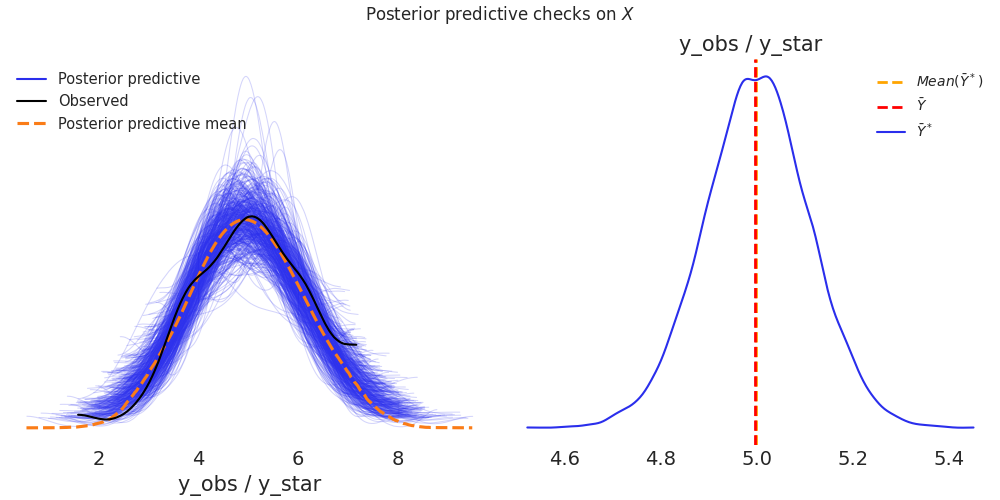
\includegraphics[width=.75\textwidth]{img/ppc_linear}
  \caption{Posterior predictive graphical checks on a fitted model. On the left there is a comparison between the observed distribution of the response variable and the posterior predictive distribution of the approximate sampled responses, while the distribution of the average of the posterior predictive responses is depicted on the right.}\label{fig:ppc}
\end{figure}
